%!TEX program = xelatex
\documentclass[12pt, a4paper]{article}

\usepackage[dvipsnames]{xcolor}

\usepackage{fancyhdr}
\usepackage{extramarks}
\usepackage{amsmath}
\usepackage{empheq}
\usepackage{amsthm}
\usepackage{amsfonts}
\usepackage{tikz}
\usepackage{tikz-3dplot}
\usepackage[plain]{algorithm}
\usepackage{algpseudocode}

\usepackage{ctex}
\usepackage{upgreek}
\usepackage{indentfirst}
\usepackage{wrapfig}
\usepackage{subfigure}
\usepackage{pgfplots}
\usepgfplotslibrary{patchplots}
\usepgfplotslibrary{colormaps}
\usepgfplotslibrary{colorbrewer}
\pgfplotsset{compat=1.18}
\usetikzlibrary{automata,positioning,shapes.geometric,arrows.meta,patterns,calc}
\numberwithin{equation}{section}
\CTEXoptions[today=old]

%
% Basic Document Settings
%

\topmargin=-0.25in
\evensidemargin=0in
\oddsidemargin=0in
\textwidth=6.5in
\textheight=9.2in
\headsep=0.25in

\linespread{1.1}

\pagestyle{fancy}
\lhead{\hmwkAuthorName}
\chead{\hmwkClass : \hmwkTitle}
\rhead{\firstxmark}
\lfoot{\lastxmark}
\cfoot{\thepage}

\renewcommand\headrulewidth{0.4pt}
\renewcommand\footrulewidth{0.4pt}

\setlength{\parindent}{2em}  % 2em代表首行缩进两个字符

%
% Create Problem Sections
%

\newcommand{\enterProblemHeader}[1]{
    \nobreak\extramarks{}{Problem \arabic{#1} continued on next page\ldots}\nobreak{}
    \nobreak\extramarks{Problem \arabic{#1} (continued)}{Problem \arabic{#1} continued on next page\ldots}\nobreak{}
}

\newcommand{\exitProblemHeader}[1]{
    \nobreak\extramarks{Problem \arabic{#1} (continued)}{Problem \arabic{#1} continued on next page\ldots}\nobreak{}
    \stepcounter{#1}
    \nobreak\extramarks{Problem \arabic{#1}}{}\nobreak{}
}

% \setcounter{secnumdepth}{0}
\newcounter{partCounter}
\newcounter{homeworkProblemCounter}
\setcounter{homeworkProblemCounter}{0}
% \nobreak\extramarks{Problem \arabic{homeworkProblemCounter}}{}\nobreak{}

%
% Homework Problem Environment
%
% This environment takes an optional argument. When given, it will adjust the
% problem counter. This is useful for when the problems given for your
% assignment aren't sequential. See the last 3 problems of this template for an
% example.
%
\newenvironment{homeworkProblem}[1][-1]{
    \ifnum#1>0
        \setcounter{homeworkProblemCounter}{#1}
    \fi
    \section{Problem \arabic{homeworkProblemCounter}}
    \setcounter{partCounter}{1}
    \enterProblemHeader{homeworkProblemCounter}
}{
    \exitProblemHeader{homeworkProblemCounter}
}

%
% Homework Details
%   - Title
%   - Due date
%   - Class
%   - Section/Time
%   - Instructor
%   - Author
%

\newcommand{\hmwkTitle}{The Method of Differentiation of Multivariate Functions and Its Applications}
\newcommand{\hmwkClass}{Advanced Mathematics}
\newcommand{\hmwkClassTime}{}
\newcommand{\myUniversiy}{Wuhan University}
\newcommand{\hmwkAuthorName}{\textbf{Lai Wei}}

%
% Title Page
%

\title{
    \vspace{2in}
    \textmd{\textbf{\hmwkClass:\ \hmwkTitle}}\\
    \vspace{0.4in}
    \large{\textit{\myUniversiy}}
    \vspace{3in}
}

\author{\hmwkAuthorName}
\date{\today}

\renewcommand{\part}[1]{\textbf{\large Part \Alph{partCounter}}\stepcounter{partCounter}\\}

%
% Various Helper Commands
%

% Useful for algorithms
\newcommand{\alg}[1]{\textsc{\bfseries \footnotesize #1}}

% % For derivatives
% \newcommand{\deriv}[1]{\frac{\mathrm{d}}{\mathrm{d}x} (#1)}

% For partial derivatives
% \newcommand{\pderiv}[2]{\frac{\partial}{\partial #1} (#2)}

% Integral dx
\newcommand{\dx}{\mathrm{d}x}

% Alias for the Solution section header
\newcommand{\solution}{\textbf{\large Solution}}

% Probability commands: Expectation, Variance, Covariance, Bias
\newcommand{\E}{\mathrm{E}}
\newcommand{\Var}{\mathrm{Var}}
\newcommand{\Cov}{\mathrm{Cov}}
\newcommand{\Bias}{\mathrm{Bias}}

% 我的newcommand
\newcommand{\degree}{^{\circ}}
\newcommand{\arrow}{-{Stealth[length=4mm,width=2mm]}}
\newcommand{\rmd}{\mathrm{d}}
\newcommand{\deriv}[2]{\frac{\rmd #1}{\rmd #2}}
\renewcommand{\parallel}{\mathrel{/\mskip-2.5mu/}}
\newcommand{\pderiv}[2]{\frac{\partial #1}{\partial #2}}
\newcommand{\parallelogram}{
	\mathord
    {\text
        {
			\tikz[baseline]
			\draw (0,.1ex) -- (.8em,.1ex) -- (1em,1.6ex) -- (.2em,1.6ex) -- cycle;
        }
    }
}

\begin{document}

\maketitle

\pagebreak

% 设置页码格式是罗马数字
\pagenumbering{roman}

% 生成目录
\tableofcontents

\pagebreak

% 设置页码格式是阿拉伯数字
\pagenumbering{arabic}

\pagebreak

\section{多元函数的基本概念}

\subsection{平面点集}

\subsubsection{坐标平面}

    建立了坐标系的平面。二元有序实数组\(\left(x,y\right)\)
    的全体,即$\mathbf{R}^2=\mathbf{R} \times \mathbf{R}=\{(x, y) 
    \mid x, y \in \mathbf{R}\}$就表示坐标平面。

\subsubsection{平面点集}

    坐标平面上具有某种性质\(P\)的点的几何,称作平面点集,记作

    \[
        E = \left\{\left(x,y\right) \mid \left(x,y\right)
        \text{具有某种性质}P\right\}
    \]

\subsubsection{邻域}

    设\(P_{0}\left(x_0,y_0\right)\)是\(xOy\)平面上一点,
    \(\delta\)是某一正数,与点\(P_{0}\left(x_0,y_0\right)\)
    距离小于\(\delta\)的点\(P\left(x,y\right)\)的全体,称为
    \(P_{0}\)的\(\delta\)邻域,记作\(U\left(P_0,\delta\right)\),
    即

    \[
        U\left(P_0,\delta\right) = \left\{\left(x,y\right)
        \mid \left|PP_0\right| < \delta\right\}
    \]

    或

    \[
        U\left(P_0,\delta\right) = \left\{\left(x,y\right)
        \mid \sqrt{\left(x-x_0\right)^2 + \left(y-y_0\right)^2} < \delta\right\}
    \]

    \textbf{注意}

    \begin{enumerate}
        \item 点\(P_0\)的去心邻域,记作$\stackrel{\circ}{U}\left(P_0, \delta\right)$,即
            $$
                \stackrel{\circ}{U}\left(P_0, \delta\right)=\left\{P\mid0<\left|P P_0\right|<\delta\right\}
            $$
        \item 若不强调\(\delta\),也可记作\(U\left(P_0\right)\),
            \(\stackrel{\circ}{U}\left(P_0\right)\)
    \end{enumerate}

    利用点与点集的关系,可知

    若有一点\(P \in \mathbf{R}^2\),任意点集\(E \subset \mathbf{R}^2\)

    \begin{enumerate}
        \item 内点:\(\exists U\left(P\right)\),使\(U\left(P\right) \subset E\),
            则\(P\)为\(E\)的内点。
        \item 外点:\(\exists U\left(P\right)\),使\(U\left(P\right) \cap E = \phi\),
            则\(P\)为\(E\)的内点。
        \item 边界点:\(\forall U\left(P\right)\),若\(U\left(P\right)\)
            即有属于\(E\)的点,又有不属于\(E\)的点,则\(P\)为\(E\)的边界点。
        \item \(E\)的边界:\(E\)的边界点的全体,记作\(\partial E\)
    \end{enumerate}

\subsubsection{聚点}

    如果对于任意给定的\(\delta>0\),点\(P\)的去心邻域
    \(\stackrel{\circ}{U}\left(P,\delta\right)\)内总有\(E\)
    中的点,那么称\(P\)是\(E\)的聚点。

    例如,若\(E = \left\{\left(x,y\right) \mid
    1 < x^2+y^2 \leq 2\right\}\)。则\(x^2+y^2=1\)
    和\(x^2+y^2=2\)都是\(E\)的聚点。

\subsubsection{由点集所属类的特征分类}

    \begin{enumerate}
        \item 开集:若点集\(E\)中的所有点都是\(E\)的内点,则称\(E\)为开集;
        \item 闭集:若点集\(E\)的边界\(\partial E \in E\),则称\(E\)为闭集。
    \end{enumerate}

    例如,\(\left\{\left(x,y\right) \mid 1 < x^2+y^2 < 2\right\}\)为开集,
    \(\left\{\left(x,y\right) \mid 1 \leq x^2+y^2 \leq 2\right\}\)为闭集,\\
    \(\left\{\left(x,y\right) \mid 1 < x^2+y^2 \leq 2\right\}\)

    \begin{figure}[htbp]
        \centering
        \subfigure[]
        {
            \begin{minipage}[b]{.3\linewidth}
                \centering
                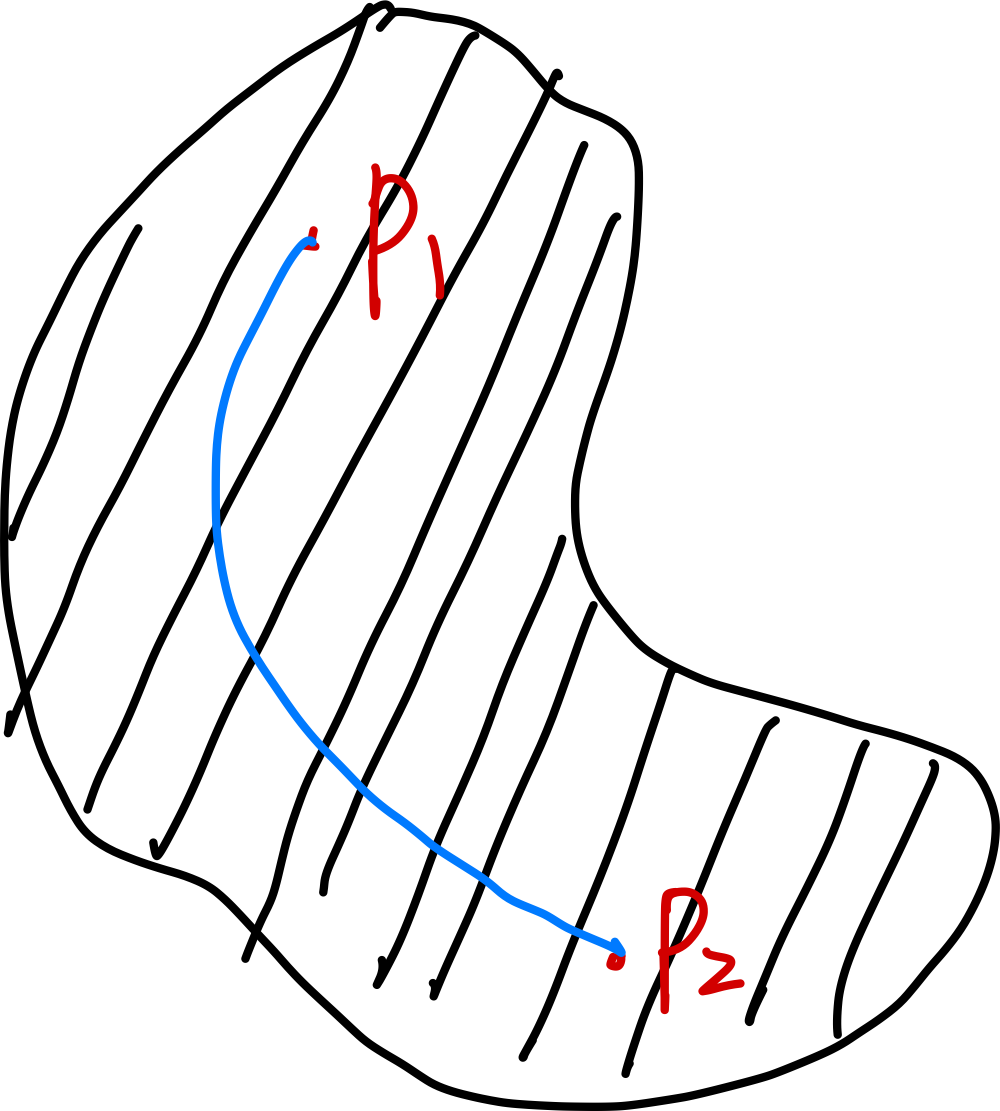
\includegraphics[scale=0.08]{"Chapter 09 images/pic1.png"}
            \end{minipage}
        }
        \subfigure[]
        {
             \begin{minipage}[b]{.3\linewidth}
                \centering
                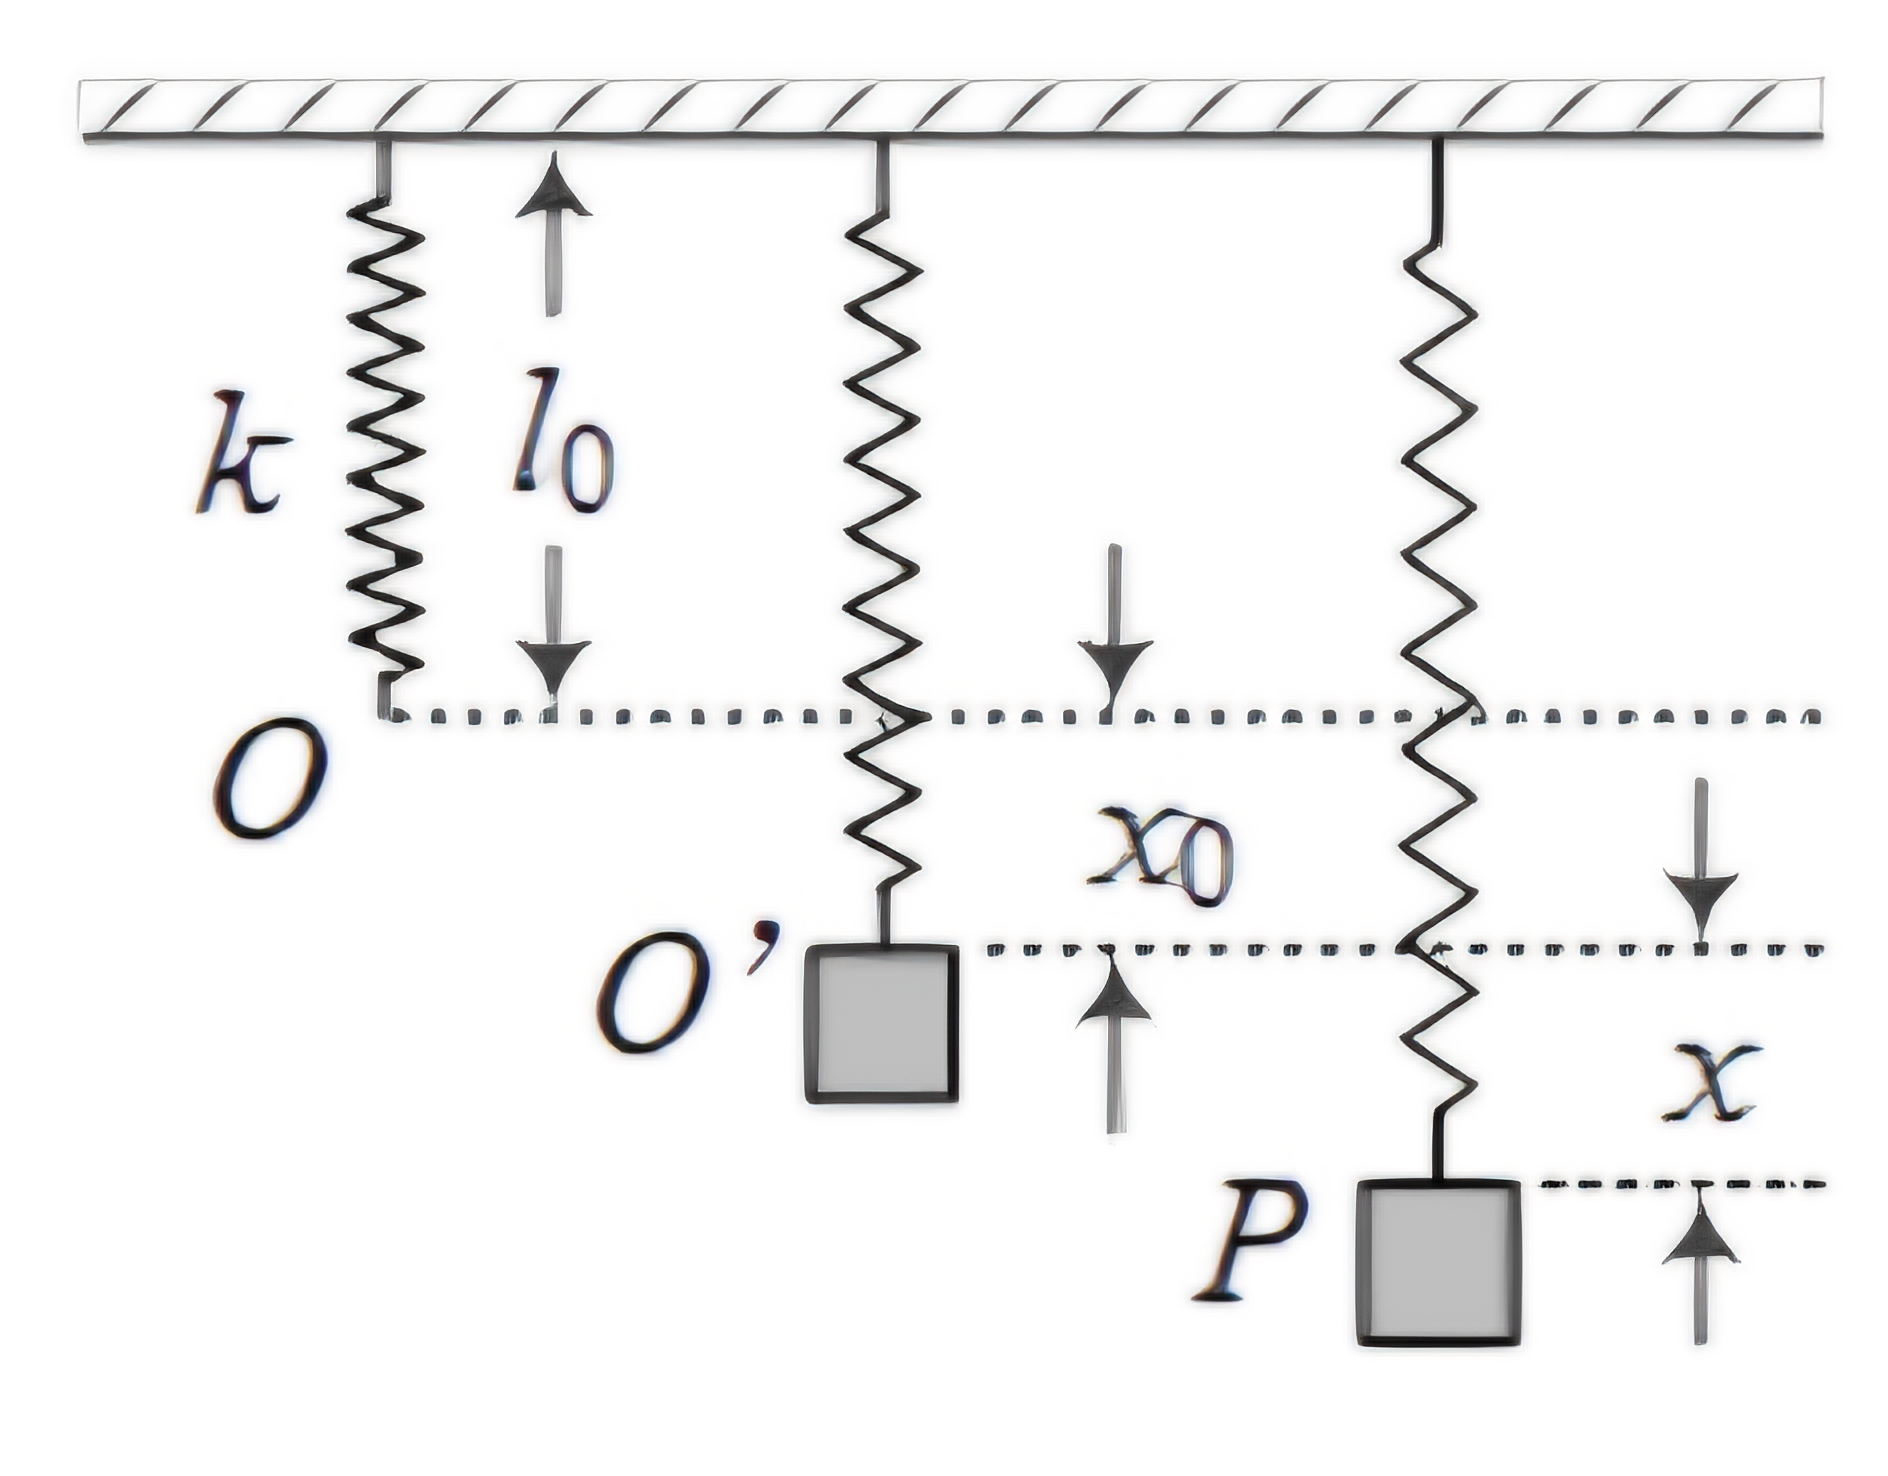
\includegraphics[scale=0.08]{"Chapter 09 images/pic2.jpg"}
            \end{minipage}
        }
    \end{figure}

    \begin{enumerate}
        \item 连通集:如上图(a);
        \item 非连通集:如上图(b)。
    \end{enumerate}

    \begin{enumerate}
        \item 开区域(也简称区域):连通的开集;
        \item 闭区域:开区域连同其边界一起构成的点集。
    \end{enumerate}

    如\(\left\{\left(x,y\right) \mid 1 < x^2+y^2 < 2\right\}\)
    为(开)区域;\(\left\{\left(x,y\right) \mid 1 \leq x^2+y^2 \leq 2\right\}\)
    为闭区域。

    \begin{enumerate}
        \item 有界集:对于集合\(E\),若\(\exists r > 0\),使\(E \subset U\left(0,r\right)\),
            则称\(E\)是有界的。(就是说能找到一个“圆”把集合\(E\)包裹起来)
        \item 无界集:若一个集合不是有界集,则称其为无界集。
    \end{enumerate}

    \begin{figure}[htbp]
        \centering
        \subfigure
        {
        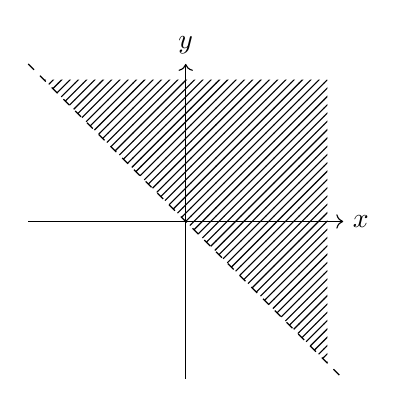
\begin{tikzpicture}
            \coordinate[label=right:$x$] (x) at (2,0);
            \coordinate[label=above:$y$] (y) at (0,2);
            \draw[->] (-2,0) -- (x);
            \draw[->] (0,-2) -- (y);
            \draw[dashed, domain=-2:2] plot(\x,{-\x});
            \fill[pattern=north east lines] (-1.8,1.8) -- (1.8,1.8) -- (1.8,-1.8);
        \end{tikzpicture}
        }
        \subfigure
        {
        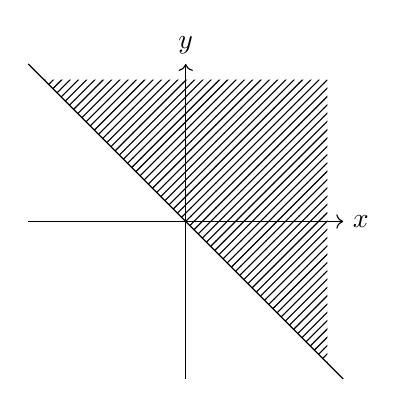
\begin{tikzpicture}
            \coordinate[label=right:$x$] (x) at (2,0);
            \coordinate[label=above:$y$] (y) at (0,2);
            \draw[->] (-2,0) -- (x);
            \draw[->] (0,-2) -- (y);
            \draw[domain=-2:2] plot(\x,{-\x});
            \fill[pattern=north east lines] (-1.8,1.8) -- (1.8,1.8) -- (1.8,-1.8);
        \end{tikzpicture}
        }
    \end{figure}

    例如,\(\left\{\left(x,y\right) \mid x + y > 0\right\}\)为无界开区域;
    \(\left\{\left(x,y\right) \mid x + y \geq 0\right\}\)为无界闭区域。

\subsection{多元函数的概念}

    \subsubsection{二元函数}

    设\(D\)是\(\mathbf{R}^2\)的一个非空子集,称映射\(f: D \rightarrow \mathbf{R}\)为定义在\(D\)上的二元函数,
    通常记为

    \begin{equation}
        z = f\left(x,y\right),\; \left(x,y\right) \in D
    \end{equation}

    或

    \begin{equation}
        z = f\left(P\right),\; P \in D
    \end{equation}

    \subsubsection{值域}

    上述定义中,与自变量\(x\)和y\(\)的一对值(即二元有序实数组)\(\left(x,y\right)\) 相对应的因变量\(z\)的值,
    也称为\(f\)在点\(\left(x,y\right)\)处的函数值,记作\(f\left(x,y\right)\),即\(z=f\left(x,y\right)\)
    函数值\(f\left(x,y\right)\)的全体所构成的集合为函数\(f\)的值域,记作\(f\left(D\right)\),即

    \begin{align}
        f\left(D\right) = \left\{z \mid z=f\left(x,y\right),\; \left(x,y\right) \in D\right\}
    \end{align}

    \subsubsection{推广}

    三元函数:\(u = f\left(x,y,z\right),\; \left(x,y,z\right) \in D\);

    \(n\)元函数:\(u = f\left(x_1,x_2,x_3,\ldots,x_n\right),\; \left(x_1,x_2,x_3,\ldots,x_n\right) \in D\)

    \subsubsection{自然定义域}

    使算式有意义的点的集合。
    
    例如\(z = \ln \left(x+y\right)\)的自然定义域为
    \(D = \left\{\left(x,y\right) \mid x + y > 0\right\}\)。\(z = \arcsin \left(x+y\right)\)
    的自然定义域为\(D = \left\{\left(x,y\right) \mid x^2 + y^2 \leq 1\right\}\)。

    \subsubsection{二元函数的图形}

    设函数\(z=f\left(x,y\right)\)的定义域为\(D\)。对于任意取定的点\(P(x,y) \in D\),
    对应的函数值为\(z=f\left(x,y\right)\)。这样,以\(x\)为横坐标,\(y\)为纵坐标和
    \(z=f\left(x,y\right)\)为竖坐标在空间就确定一点\(M\left(x,y,z\right)\)。
    当\(x,y\)遍取\(D\)上的一切点时,得到一个空间点集

    \begin{align}
        \left\{\left(x,y,z\right) \mid z=f\left(x,y\right),\; \left(x,y\right) \in D\right\}
    \end{align}
    
    这个点集称为二元函数\(z=f\left(x,y\right)\)的图形,通常我们也说二元函数的图形是一张曲面。

    例如,由空间解析几何知道,线性函数$z=ax+by+c$
    的图形是一张平面,而函数$z=x^2+y^2$的图形是旋转抛物面。

\subsection{多元函数的极限}

    如果在\(P\left(x,y\right) \rightarrow P_0\left(x_0,y_0\right)\)(即\(\left|PP_0\right| =
    \sqrt{\left(x-x_0\right)^2 + \left(y-y_0\right)^2} \rightarrow 0\))过程中,对应的函数值
    无限接近于一个确定的常数\(A\),那么就说\(A\)是函数\(f\left(x,y\right)\)当
    \(\left(x,y\right) \rightarrow \left(x_0,y_0\right)\)时的极限。

    \textbf{定义}:“\(\varepsilon - \delta\)”语言

    设二元函数 $f(P)=f(x, y)$ 的定义域为 $D$,$P_0\left(x_0, y_0\right)$
    是$D$的聚点。如果存在常数$A$,对于任意给定的正数$\varepsilon$,总存在正数$\delta$,
    使得当点$P(x, y) \in D \cap \ddot{U}\left(P_0, \delta\right)$ 时,都有

    \begin{equation}
        \left|f(P)-A\right|=\left|f(x, y)-A\right|<\varepsilon
    \end{equation}

    成立,那么就称常数\(A\)为函数\(f\left(x,y\right)\)当\(\left(x,y\right) \rightarrow \left(x_0,y_0\right)\)
    的极限,记作

    \begin{equation}
        \lim _{P \rightarrow P_0} f(P)=A \quad
    \end{equation}

    或

    \begin{equation}
        f(P) \rightarrow A\left(P \rightarrow P_0\right)
    \end{equation}

    \textbf{注意}:

    \begin{enumerate}
        \item \(P_0\)是\(D\)的聚点;
        \item 证明过程中,核心在于寻找\(\delta = \delta\left(\varepsilon\right)\);
        \item 与一元函数不同,\(P \rightarrow P_0\)是指\(P\)以任何方式趋近\(P_0\);
        \item 若\(P\)以不同方式趋近于\(P_0\),\(f\left(p\right)\)趋近于不同值,则可以断定\(f\left(p\right)\)当\(P \rightarrow P_0\)时的极限不存在。
    \end{enumerate}

\subsection{多元函数的连续性}

\subsubsection{连续性的定义}

    设二元函数\(f\left(P\right) = f\left(x,y\right)\)的定义域为\(D\),\(P_0\left(x_0,y_0\right)\)
    为\(D\)的聚点,且\(P_0 \in D\),如果

    \begin{align}
        \lim_{\left(x,y\right) \rightarrow \left(x_0,y_0\right)}f\left(x,y\right) = f\left(x_0,y_0\right)
    \end{align}

    那么称\(f\left(P\right)\)在点\(P_0\left(x_0,y_0\right)\)连续。

    \textbf{注意}:若\(f\left(x,y\right)\)在\(D\)的每一个点都是连续的,则称\(f\left(x,y\right)\)在上\(D\)为连续的。

\subsubsection{间断点的定义}

    设二元函数\(f\left(x,y\right)\)的定义域为\(D\),\(P_0\left(x_0,y_0\right)\)
    为\(D\)的聚点,如果函数\(f\left(x,y\right)\)在\(P_0\left(x_0,y_0\right)\)\\
    点不连续,那么就称\(P_0\left(x_0,y_0\right)\)为函数\(f\left(x,y\right)\)的间断点。

\subsubsection{连续函数的运算}

    一元函数中关于极限的运算法划,对于多元函数仍然适用。根据多元函数的极限运算法则,
    可以证明多元连续函数的和、差、积仍为连续函,连续函数的商在分母不为零出仍连续;
    多元连续函数的复合函数仍然是连续函数。

\subsubsection{多元初等函数}

    与一元初等函数相类似,多元初等函数是指可用一个式子表示的多元函数,这
    个式子是由常数及具有不同自变量的一元基本初等函数经过有限次的四则运算和
    复合运算而得到的。例如\(\frac{x + x^2 + y^2}{1+y^2}\)、
    \(\sin\left(x+y\right)\)、\(e^{x^2 + y^2 + z^2}\)等都是多元初等函数。
    
\subsubsection{有界闭区域上多元函数连续函数的性质}

    \begin{enumerate}
        \item (\textbf{有界性与最大值最小值定理})有界闭区域\(D\)上连续的多元函数,必定在\(D\)上有
            上界,且能取得它的最大值和最小值。\\
            也就是说,若\(P\)在有界闭区域\(D\)上连续,则必定存在常数\(M>0\),使得对一切\(P \in D\)
            有\(\left|f\left(D\right)\right| \leq M\);且存在\(P_1,P_2 \in D\),使得
            $$
                f\left(P_1\right)=\max \{f(P) \mid P \in D\},\; f\left(P_2\right)=\min \{f(P) \mid P \in D\}
            $$
        \item (\textbf{介值定理})在有界闭区域\(D\)上连续的多元函数必取得介于最大值和最小值之间的任何值。
        \item (\textbf{一致连续性定理})在有界闭区域\(D\)上连续的多元函数必定在\(D\)上一致连续。\\
            也就是说,若\(f\left(P\right)\)在有界闭区域\(D\)上连续,则对任意给定的正数\(\varepsilon\),
            总存在正数\(\delta\),使得对于\(D\)上任意两点\(P_1\)、\(P_2\),只要当\(\left|P_1P_2\right| < \varepsilon\)
            时,都有
            $$
                \left|f\left(P_1\right) - f\left(P_2\right)\right| < \varepsilon
            $$
            成立。
    \end{enumerate}

\subsection{例题}

\subsubsection{Problem 1}

    设\(f\left(x,y\right) = \left(x^2+y^2\right)\sin \dfrac{1}{x^2+y^2}\),求证

    \[
        \lim_{\left(x,y\right) \rightarrow \left(x_0,y_0\right)}f\left(x,y\right) = 0
    \]
    \vspace{1em}

    \textbf{Solution}
    \vspace{1em}

    \(f\left(x,y\right)\)的定义域为\(D = \mathbf{R}^2 \backslash \left\{\left(0,0\right)\right\}\),
    点\(O\left(0,0\right)\)为\(D\)的聚点。

    而$\left|f(x, y)-0\right|=\left|f(x, y)\right|=
    \left|\left(x^2+y^2\right) \sin \dfrac{1}{y+x^2}\right| \leq x^2+y^2$

    对\(\forall \varepsilon > 0\)要使$\left|f(x, y)-0\right| \leq x^2+y^2 < \varepsilon$
    成立,取$\delta = \sqrt{\varepsilon}$,则\(0 < \sqrt{x^2+y^2} < \delta\)时,
    有$\left|f(x, y)-0\right| < \varepsilon$。

    于是
    
    \[
        \lim_{\left(x,y\right) \rightarrow \left(x_0,y_0\right)}f\left(x,y\right) = 0
    \]

\subsubsection{Problem 2}

    求证函数

    $$
        f(x, y)= \begin{cases}\dfrac{x y}{x^2+y^2}, & x^2+y^2 \neq 0 \\ 0, & x^2+y^2=0\end{cases}
    $$

    当$\left(x,y\right) \rightarrow \left(0,0\right)$时的极限不存在。
    \vspace{1em}

    \textbf{Solution}
    \vspace{1em}

    显然,当\(P\left(x,y\right)\)沿\(x\)轴趋近于点\(\left(0,0\right)\)时,

    $$
        \lim_{\substack{x, y \rightarrow(0,0) \\ y=0}} f(x, y)=\lim_{x \rightarrow 0} f(x, 0)=\lim _{x \rightarrow 0} 0=0 ;
    $$

    当\(P\left(x,y\right)\)沿直线\(y = kx\)趋近于点\(\left(0,0\right)\)时,

    $$
        \lim_{\substack{(x, y) \rightarrow(0,0) \\ y=k x}} \frac{x y}{x^2+y^2}=\lim_{x \rightarrow 0} \frac{k x^2}{x^2+k^2 x^2}=\frac{k}{1+k^2},
    $$

    显然它是随着\(k\)的值的不同而改变的。

    所以原函数当$\left(x,y\right) \rightarrow \left(0,0\right)$时的极限不存在。

\subsubsection{Problem 3}

    求

    $$
        \lim_{\left(x,y\right) \rightarrow \left(0,2\right)} \frac{\sin\left(xy\right)}{x}
    $$
    \vspace{1em}

    \textbf{Solution}
    \vspace{1em}

    \begin{align*}
        \text{原式} &= \lim_{\left(x,y\right) \rightarrow \left(0,2\right)} \frac{\sin\left(xy\right)}{xy} \cdot y \\
        &=\lim_{xy \rightarrow 0} \frac{\sin\left(xy\right)}{xy} \cdot \lim_{y\rightarrow 2}y \\
        &= 1 \times 2 \\
        &= 2
    \end{align*}

\section{偏导数}

\subsection{偏导数的定义及其计算法}

\subsubsection{定义}

    设函数\(z=f\left(x,y\right)\)在点\(\left(x_0,y_0\right)\)的某一邻域内有定义,
    当\(y\)固定在\(y_0\)而\(x\)在\(x_0\)处有增量\\ \(\Delta x\)时,相应的函数有增量

    $$
        f\left(x_0+\Delta x, y_0\right)-f\left(x_0, y_0\right)
    $$

    如果

    \begin{equation}
        \lim _{\Delta x \rightarrow 0} \frac{f\left(x_0+\Delta x, y_0\right)-f\left(x_0, y_0\right)}{\Delta x}
        \label{9-4-1}
    \end{equation}

    存在,那么称此极限为函数\(z=f\left(x,y\right)\)在点\(\left(x_0,y_0\right)\)处\textbf{对\(x\)的偏导数},记作

    $$
        \left.\frac{\partial z}{\partial x}\right|_{\substack{x=x_0 \\ y=y_0}},\;
        \left.\frac{\partial f}{\partial x}\right|_{\substack{x=x_0 \\ y=y_0}},\;
        \left.z_x\right|_{\substack{x=x_0 \\ y=y_0}}\; \text{或}\;
        f_x\left(x_0, y_0\right) \text {. (1) }
    $$

    例如,方程\ref{9-4-1}可以表为

    \begin{equation}
        f_x\left(x_0, y_0\right)=\lim _{\Delta x \rightarrow 0} \frac{f\left(x_0+\Delta x, y_0\right)-f\left(x_0, y_0\right)}{\Delta x}
    \end{equation}

    类似地,函数\(z=f\left(x,y\right)\)在点\(\left(x_0,y_0\right)\)处\textbf{对\(y\)的偏导数}定义为

    \begin{equation}
        \lim _{\Delta y \rightarrow 0} \frac{f\left(x_0, y_0+\Delta y\right)-f\left(x_0, y_0\right)}{\Delta y}
    \end{equation}

    记作

    $$
        \left.\frac{\partial z}{\partial y}\right|_{\substack{x=x_0 \\ y=y_0}},\;
        \left.\frac{\partial f}{\partial y}\right|_{\substack{x=x_0 \\ y=y_0}},\;
        \left.z_y\right|_{\substack{x=x_0 \\ y=y_0}}\; \text{或}\;
        f_y\left(x_0, y_0\right)
    $$

    如果函数\(z=f\left(x,y\right)\)在区域\(D\)内每一点\(\left(x,y\right)\)处对\(x\)的偏导数都存在,
    那么这个偏导数就是\(x\)、\(y\)的函数,它就称为函数\(z=f\left(x,y\right)\)\textbf{对自变量\(x\)的偏导函数},
    记作

    $$
        \pderiv{z}{x},\;
        \pderiv{f}{x},\;
        z_x\; \text{或}\;
        f_x\left(x, y\right)
    $$

    类似地,可以定义函数\(z=f\left(x,y\right)\)\textbf{对自变量\(y\)的偏导函数},
    记作

    $$
        \pderiv{z}{y},\;
        \pderiv{f}{y},\;
        z_y\; \text{或}\;
        f_y\left(x, y\right)
    $$

    由概念可知,函数\(z=f\left(x,y\right)\)在点\(\left(x_0,y_0\right)\)处对\(x\)的偏导数
    \(f_x\left(x_0, y_0\right)\)显然就是偏导函数\(f_x\left(x, y\right)\)在点\(\left(x_0,y_0\right)\)
    处的函数值;\(f_y\left(x_0, y_0\right)\)就是偏导函数\(f_y\left(x, y\right)\)在点
    \(\left(x_0,y_0\right)\)处的函数值。

\subsubsection{偏导数的求法}

    求\(\pderiv{f}{x}\)时,只要把\(y\)暂时看作常量而对\(x\)求导数;
    求\(\pderiv{f}{y}\)时,只要把\(x\)暂时看作常量而对\(y\)求导数。

    推广:三元函数\(u=f\left(x,y,z\right)\)在点\(\left(x,y,z\right)\)
    处对\(x\)的偏导数定义为

    \begin{equation}
        f_x(x, y, z)=\lim _{\Delta x \rightarrow 0} \frac{f(x+\Delta x, y, z)-f(x, y, z)}{\Delta x}
    \end{equation}

    \textbf{注意}:

    \begin{enumerate}
        \item \(z=f\left(x,y\right)\)的偏导数有2个:\(\pderiv{z}{x}\) 、\(\pderiv{z}{y}\),
            \(u=f\left(x,y,z\right)\)的偏导数有3个:\(\pderiv{u}{x}\) 、\(\pderiv{u}{y}\) 、\(\pderiv{u}{z}\);
        \item \(\pderiv{z}{x}\)是一个整体、一个符号。
    \end{enumerate}


\subsubsection{偏导数的几何意义}

    \begin{wrapfigure}{r}{4cm}
        \centering
        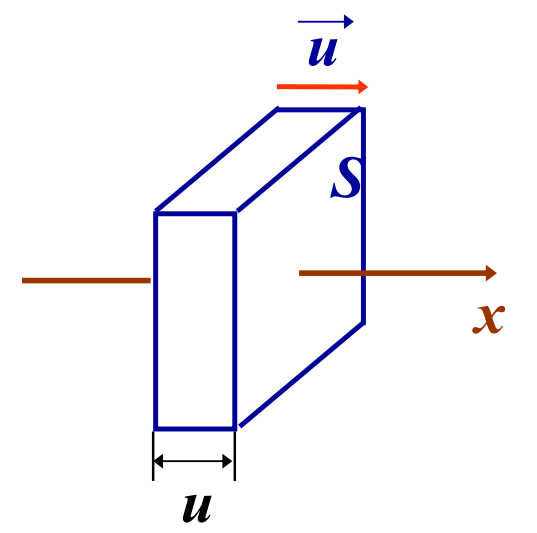
\includegraphics[scale=0.15]{"Chapter 09 images/pic3.jpg"}
        % \caption{}
        \label{pic9-3}
    \end{wrapfigure}

    设\(M_0\left(x_0,y_0,z_0\right)\)为曲面\(z=f\left(x,y\right)\)上的一点,
    过\(M_0\)作平面\(y=y_0\),截此曲面得一平面,此曲线在平面\(y=y_0\)上的方程为
    \(z=f\left(x,y_0\right)\),
    则导数\(\left.\dfrac{\rmd}{\rmd x} f\left(x,y_0\right)\right|_{x=x_0}\),
    即偏导数\(f_x\left(x_0,y_0\right)\),就是这曲线在点\(M_0\)处的切线\(M_0T_x\)
    对\(x\)轴的斜率(如右图所示)。同样,偏导数\(f_y\left(x_0,y_0\right)\)
    的几何意义是曲面被平面\(x=x_0\)所截得的曲线在点\(M_0\)处的切线\(M_0T_y\)
    对\(y\)轴的斜率。
    \vspace{1em}

    \textbf{注意}:

    对多元函数,若函数连续,则偏导数\textbf{不}一定存在;若偏导数存在,
    则函数也\textbf{不}一定连续。例如,函数

    $$
        z=f(x, y)= \begin{cases}\frac{x y}{x^2+y^2}, & x^2+y^2 \neq 0 \\ 0, & x^2+y^2=0\end{cases}
    $$

    在\(\left(0,0\right)\)处是不连续的,而\(f_x\left(0,0\right)=0\),\(f_y\left(0,0\right)=0\),
    即函数在\(\left(0,0\right)\)处的偏导数存在。

\subsection{高阶偏导数}

\end{document}
